% Diagrama 4 — Proceso general de negocio (v2)
% =====================================================================
%  estilo.tex — sistema visual común de los diagramas RedPepper
%  Se incluye desde cada figura (documento independiente).
% =====================================================================
\documentclass[11pt,tikz,border=6pt]{standalone}

\usepackage[utf8]{inputenc}
\usepackage[T1]{fontenc}
\usepackage{lmodern}
\usepackage{helvet}
\renewcommand{\familydefault}{\sfdefault}

\usepackage{tikz}
\usetikzlibrary{positioning,arrows.meta,shapes.geometric,fit,backgrounds,calc}

% --- Paleta por rol (tonos suaves, legibles en impresión) ---------------
\definecolor{cCliente}{HTML}{FFF1D6}
\definecolor{bCliente}{HTML}{B8860B}
\definecolor{cCaja}{HTML}{E4F2E1}
\definecolor{bCaja}{HTML}{3E7D3A}
\definecolor{cSistema}{HTML}{E3ECF9}
\definecolor{bSistema}{HTML}{2F5D9E}
\definecolor{cCocina}{HTML}{FBE5E3}
\definecolor{bCocina}{HTML}{A33B33}
\definecolor{cAdmin}{HTML}{EDEDED}
\definecolor{bAdmin}{HTML}{555555}
\definecolor{cProveedor}{HTML}{F0E7F7}
\definecolor{bProveedor}{HTML}{6A4C93}
\definecolor{cContador}{HTML}{DEF1EF}
\definecolor{bContador}{HTML}{2E7D74}

% --- Estilos ------------------------------------------------------------
\tikzset{
  proc/.style={
    draw=black!55, rounded corners=3pt, fill=white, align=center,
    font=\small,
    execute at begin node={\hyphenpenalty=10000\exhyphenpenalty=10000},
    inner sep=3.5pt, minimum height=0.95cm, text width=3.05cm
  },
  cliente/.style={proc, fill=cCliente, draw=bCliente},
  caja/.style={proc, fill=cCaja, draw=bCaja},
  sistema/.style={proc, fill=cSistema, draw=bSistema},
  cocina/.style={proc, fill=cCocina, draw=bCocina},
  admin/.style={proc, fill=cAdmin, draw=bAdmin},
  proveedor/.style={proc, fill=cProveedor, draw=bProveedor},
  contador/.style={proc, fill=cContador, draw=bContador},
  dec/.style={
    diamond, aspect=2.1, draw=black!60, fill=white, align=center,
    font=\footnotesize, inner sep=1pt, minimum width=2.6cm, minimum height=1.15cm
  },
  ini/.style={
    draw=black!60, rounded corners=14pt, fill=black!6, align=center,
    font=\footnotesize\bfseries, inner sep=5pt, minimum height=0.9cm, text width=2.6cm
  },
  flecha/.style={-{Stealth[length=2.2mm,width=1.6mm]}, draw=black!70, line width=0.7pt},
  flechad/.style={flecha, dashed},
  etiqueta/.style={font=\scriptsize, inner sep=2pt, fill=white, draw=none, text=black!75},
  banda/.style={fill=black!82, text=white, font=\small\bfseries, align=center, inner sep=4pt},
  leyenda/.style={font=\scriptsize, align=left, text=black!80}
}

% --- Encabezado y leyenda ----------------------------------------------
% #1 ancho total, #2 título, #3 y del encabezado
\newcommand{\encabezado}[3]{%
  \node[banda, minimum width=#1, minimum height=0.62cm, anchor=north west]
    at (-0.45,#3) {\strut #2};%
}
% #1 x, #2 y  (leyenda en dos filas para evitar solapamientos)
\newcommand{\leyendaRoles}[2]{%
  \begin{scope}[shift={(#1,#2)}]
    \foreach \x/\c/\b/\t in {0/cCliente/bCliente/Cliente,
                              2.7/cCaja/bCaja/Caja,
                              5.2/cSistema/bSistema/Sistema,
                              8.4/cCocina/bCocina/Cocina}{%
      \node[draw=\b, fill=\c, minimum width=0.34cm, minimum height=0.24cm,
            anchor=west] at (\x,0) {};
      \node[leyenda, anchor=west] at ({\x+0.24},0) {\t};%
    }
    \foreach \x/\c/\b/\t in {0/cAdmin/bAdmin/Administración,
                              3.4/cProveedor/bProveedor/Proveedor,
                              6.6/cContador/bContador/Contador}{%
      \node[draw=\b, fill=\c, minimum width=0.34cm, minimum height=0.24cm,
            anchor=west] at (\x,-0.42) {};
      \node[leyenda, anchor=west] at ({\x+0.24},-0.42) {\t};%
    }
  \end{scope}
}


\begin{document}
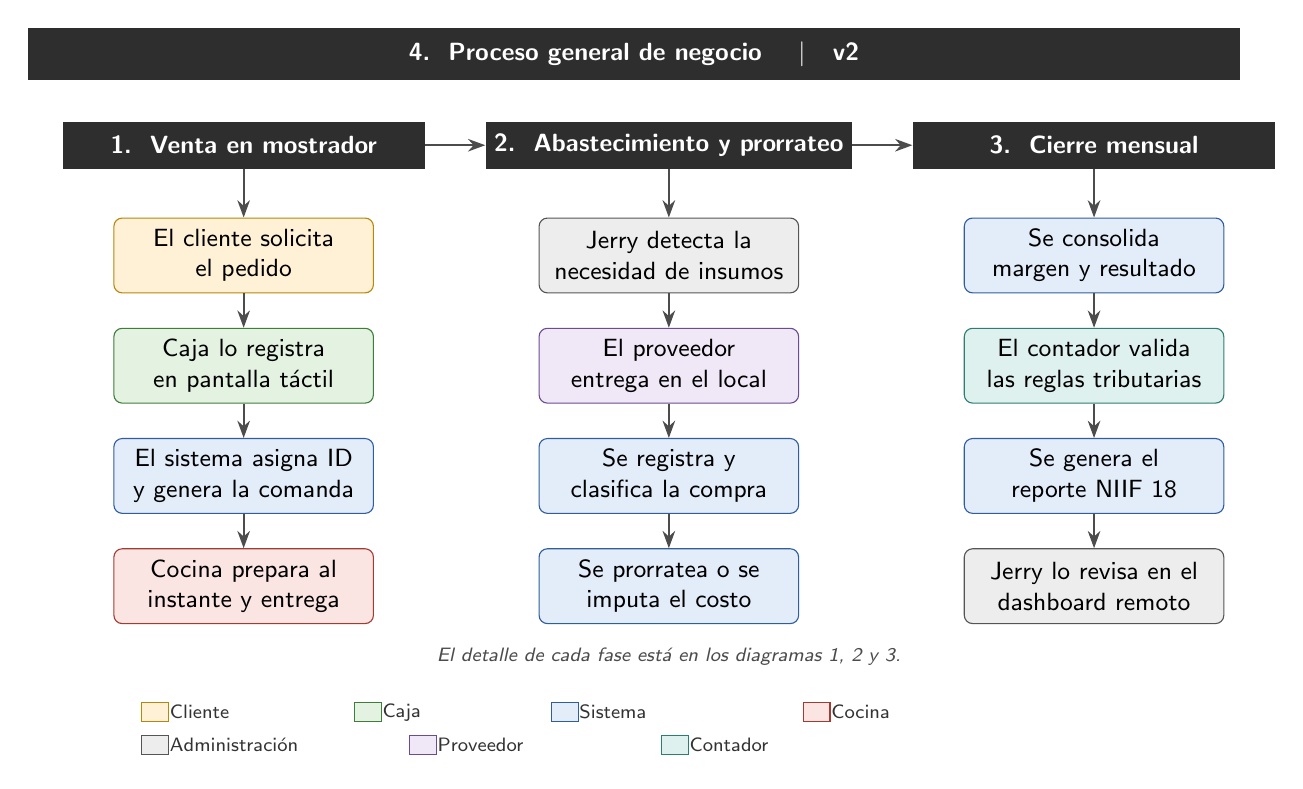
\begin{tikzpicture}[
  fase/.style={fill=black!82, text=white, font=\small\bfseries, align=center,
               minimum width=4.6cm, minimum height=0.6cm, inner sep=3pt},
  chip/.style={proc, text width=4.25cm, minimum height=1.0cm}
]

  \encabezado{15.4cm}{4.\ \ Proceso general de negocio \quad\textbar\quad v2}{1.5}

  % ---------------- Bandas de fase ----------------
  \node[fase] (f1) at (2.3,0)  {1.\ \ Venta en mostrador};
  \node[fase] (f2) at (7.7,0)  {2.\ \ Abastecimiento y prorrateo};
  \node[fase] (f3) at (13.1,0) {3.\ \ Cierre mensual};

  \draw[flecha] (f1.east) -- (f2.west);
  \draw[flecha] (f2.east) -- (f3.west);

  % ---------------- Fase 1 ----------------
  \node[chip, cliente] (a1) at (2.3,-1.4) {El cliente solicita el pedido};
  \node[chip, caja] (a2) at (2.3,-2.8) {Caja lo registra en pantalla táctil};
  \node[chip, sistema] (a3) at (2.3,-4.2) {El sistema asigna ID y genera la comanda};
  \node[chip, cocina] (a4) at (2.3,-5.6) {Cocina prepara al instante y entrega};

  % ---------------- Fase 2 ----------------
  \node[chip, admin] (b1) at (7.7,-1.4) {Jerry detecta la necesidad de insumos};
  \node[chip, proveedor] (b2) at (7.7,-2.8) {El proveedor entrega en el local};
  \node[chip, sistema] (b3) at (7.7,-4.2) {Se registra y clasifica la compra};
  \node[chip, sistema] (b4) at (7.7,-5.6) {Se prorratea o se imputa el costo};

  % ---------------- Fase 3 ----------------
  \node[chip, sistema] (c1) at (13.1,-1.4) {Se consolida margen y resultado};
  \node[chip, contador] (c2) at (13.1,-2.8) {El contador valida las reglas tributarias};
  \node[chip, sistema] (c3) at (13.1,-4.2) {Se genera el reporte NIIF 18};
  \node[chip, admin] (c4) at (13.1,-5.6) {Jerry lo revisa en el dashboard remoto};

  % ---------------- Flujos verticales ----------------
  \foreach \top/\next in {f1/a1, a1/a2, a2/a3, a3/a4,
                          f2/b1, b1/b2, b2/b3, b3/b4,
                          f3/c1, c1/c2, c2/c3, c3/c4}{
    \draw[flecha] (\top) -- (\next);
  }

  % ---------------- Nota final ----------------
  \node[font=\scriptsize\itshape, text=black!70, align=center]
    at (7.7,-6.5) {El detalle de cada fase está en los diagramas 1, 2 y 3.};

  \leyendaRoles{1.0}{-7.2}

\end{tikzpicture}
\end{document}
